\documentclass[a4paper,10pt,twoside]{cpc-hepnp}
\usepackage{multicol}
\usepackage{graphicx}
\usepackage{booktabs}
\usepackage{amssymb,bm,mathrsfs,bbm,amscd}
\usepackage[tbtags]{amsmath}
\usepackage{lastpage}
\usepackage{lineno}
\usepackage{ifpdf}
\usepackage{subfigure}
\ifpdf
   \DeclareGraphicsRule{*}{mps}{*}{}
\else
   \DeclareGraphicsRule{*}{eps}{*}{}
\fi

\linenumbers
\renewcommand{\mathstrut}{\protect\vphantom{\hat{0123456789}}}
\linespread{2} % comment this after all the revision 


\begin{document}
\fancyhead[c]{\small Chinese Physics C~~~Vol. xx, No. x (201x) xxxxxx}
\fancyfoot[C]{\small 010201-\thepage}
%\footnotetext[0]{Received 14 March 2009}


\title{ An  optimization of threshold scan of $e^+e^- \to ZH$  for Higgs spin determinatin and ISR correction at Higgs factories
\thanks{The study was partially supported by the XXXX and YYYY.}}

\author{%
          Shuang Han$^{1,2)}$\email{hans@ihep.ac.cn}%
\quad Gang Li$^{1)}$\email{li.gang@ihep.ac.cn}%
\quad Xian Zhou$^{3)}$\email{zhouxiang@ihep.ac.cn}%
}
\maketitle


\address{%
$^1$ Institute of High Energy Physics, Chinese Academy of Sciences, Beijing 100049, China\\
$^2$ Wuhan University, Hubei Province, China
}


\begin{abstract}
The cross section determination of $\sigma(e^+e^- \to ZH)$ will reach unprecedented  precision at furture Higgs factories. This makes the theoretical correction an important uncertainty in the measurement, such as initial state radiation correction and other high order electroweak corrections. Initial state radiation correction needs the experiment measurements below the present center of mass energy as input. This work study the optimal scan scheme for ISR correction to match the requirement of experimental precision. The effect of scan scheme on Higgs spin determination  is discussed as well.
\end{abstract}


\begin{keyword}
Higgs Factory, Initial state radiation, Higgs spin 
\end{keyword}

\begin{pacs}
%1---3 PACS(Physics and Astronomy Classification Scheme, http://www.aip.org/pacs/pacs.html/)
\end{pacs}

\footnotetext[0]{\hspace*{-3mm}\raisebox{0.3ex}{$\scriptstyle\copyright$}2013
Chinese Physical Society and the Institute of High Energy Physics
of the Chinese Academy of Sciences and the Institute
of Modern Physics of the Chinese Academy of Sciences and IOP Publishing Ltd}%

%\begin{multicols}{2}



\section{Introduction: $e^+e^-$ collider as a Higgs factory}\label{sec:intro}
The discovery of the Higgs boson~\cite{ref:1,ref:2} is a great milestone for the particle physics.  Precision measurements of properties of the Higgs boson are critical for the SM physics; any deviation away from the SM expectation will improve our knowledge of the elementary particles and their interactions. Based on this consideration, an $e^+e^-$ collider with high luminosity and energy is best suited for the Higgs research and several $e^+e^-$ experiments have been proposed{~\cite{ref:ilc, ref:ild, ref:cepc_det, ref:cepc_acc, ref:fccee, ref:clic}} by high energy physics community. 

At Higgs factories, usually the observables of Higgs can be measured to unprecedented precision. For example, the Born cross section, $\sigma_B(e^+e^- \to ZH)$ ( abbreviated to $\sigma_B(ZH)$ ), can be measured to 0.8\% at ILC, 0.5\% at CEPC, and 0.4\%  at FCC-$ee$, respectively.  Therefore the high order correction, including initial state radiation (ISR) and other virtual corrections, has significant contribution to the observed cross section compared with the expected precision.  Recent calculations shows that the NLO EW correction has significant contribution{~\cite{ref:jiayu, ref:yangll}}. But from the view point of experiment, ISR correction is more important, since it depends on the theoretical calculation, but the experiment itself. 


The line shape of $\sigma_B(ZH)$

This article is organized as the following. After the introduction, the ISR procedure of $e^+e^-$ experiment will be described in detail. Then the optimization of $e^+e^- \to ZH$ threshold scan scheme will be performed in order to meet the requirement of  the cross section measurement and spin determination of  Higgs boson. In the end, there will be a conclusive discussion. 

\section{$\sigma(ZH)$, ISR correction, and the Higgs spin\label{sec:presicion}}

In Higgs factories, such as CEPC, ILC, FCC-ee, and CLIC, $\sigma(ZH)$ is one of the key measurands. It is solely determined by the $C_{HZZ}$ coupling at tree level and also depends on the Higgs self-coupling at loop level, which may be altered by such couplings.  Vise versa, precise measurement of $\sigma(ZH)$  can constrain $C_{HZZ}$  and Higgs self-coupling.  

In experiment, the Born cross section is calculated with formula 
\begin{eqnarray}\label{eqn:key}
\sigma_{B} = \frac{N^{\rm obs.}}{{\mathcal L} \cdot \epsilon\cdot (1+\delta)^{\gamma} (1+\delta)^{\rm V}}~,
\end{eqnarray}
where ${\mathcal L}$ is integrated luminosity, $\epsilon$ detection efficiency, and $(1+\delta)^\gamma$  and $(1+\delta)^{V}$ the correction factors of  the ISR and other virtual correction, respectively. The ISR correction factor is calculated by the Monte Carlo (MC) generator being used to determine the detection efficiency.  The measurement requires precise calculation of ISR correction. This is done by the structure function approach, which yields the accuracy of 0.1\%~\cite{ref:isr1, ref:isr2, ref:isr3, ref:isr4, ref:isr5}. In this scheme,  the observed cross section reads 
\begin{eqnarray} \label{eqn:conv}
\sigma(s) = \int_{0}^{1-s_{th}/s} dx\tilde{\sigma}[s(1-x)]F(x,s)\,,
\end{eqnarray}
where $\sqrt{s}$ is the center of mass energy (CM) of the colliding beam, $\sqrt{s_{th}}$ is the kinematic threshold of $e^+e^- \to ZH$, and the dressed cross section 
\begin{eqnarray}\label{eqn:vp}
\tilde{\sigma} (s)= \frac{\sigma_B(s)} {(1+\delta)^{\rm V}}\,,
\end{eqnarray}
with $\sigma_B(s)$ the Born order cross-section. Through this work, $\sigma_B$ is used instead of $\tilde{\sigma}$, {\it i.e.} assuming that $(1+\delta)^{\rm V}=1$, because that the virtual correction does not depend on experiments.

According to the Eq.~\ref{eqn:conv}, it is apparent that $\sigma(ZH)$ depends not only on $F(x,s)$  but also on the line shape of $\sigma(s)$ of the region from the threshold to CM energy. The line shape has to be determined by experiment and its uncertainty contributes to the systematic uncertainty of  $\sigma(ZH)$. 

In Eq.~\ref{eqn:conv}, the radiator $F(x,s)$ 
\begin{eqnarray}\label{eqn:radiator}
F(x,s) = \beta x^{\beta -1} \delta^{V+S} + \delta^{H}~,
\end{eqnarray}
with 
\begin{eqnarray}
\beta & =& \frac{2\alpha}{\pi}\left( \ln\frac{s}{m_e^2} -1 \right)~,\\
\delta^{V+S} & =& 1 + \frac{3}{4}\beta + \frac{\alpha}{\pi}\left(\frac{\pi^2}{3}-\frac{1}{2}\right)+\beta^2\left( \frac{9}{32}-\frac{\pi^2}{12}\right)~,\\
\delta^{H} & = & -\beta\left( 1-\frac{x}{2}\right)+\frac{1}{8}\beta^2
\left[
4(2-x)\ln\frac{1}{x} - \frac{1+3(1-x)^2}{x}\ln(1-x)-6-x
\right]~.
\end{eqnarray}

\section{Optimization of threshold scan  \label{sec:optimization}}

\iffalse
\begin{center}
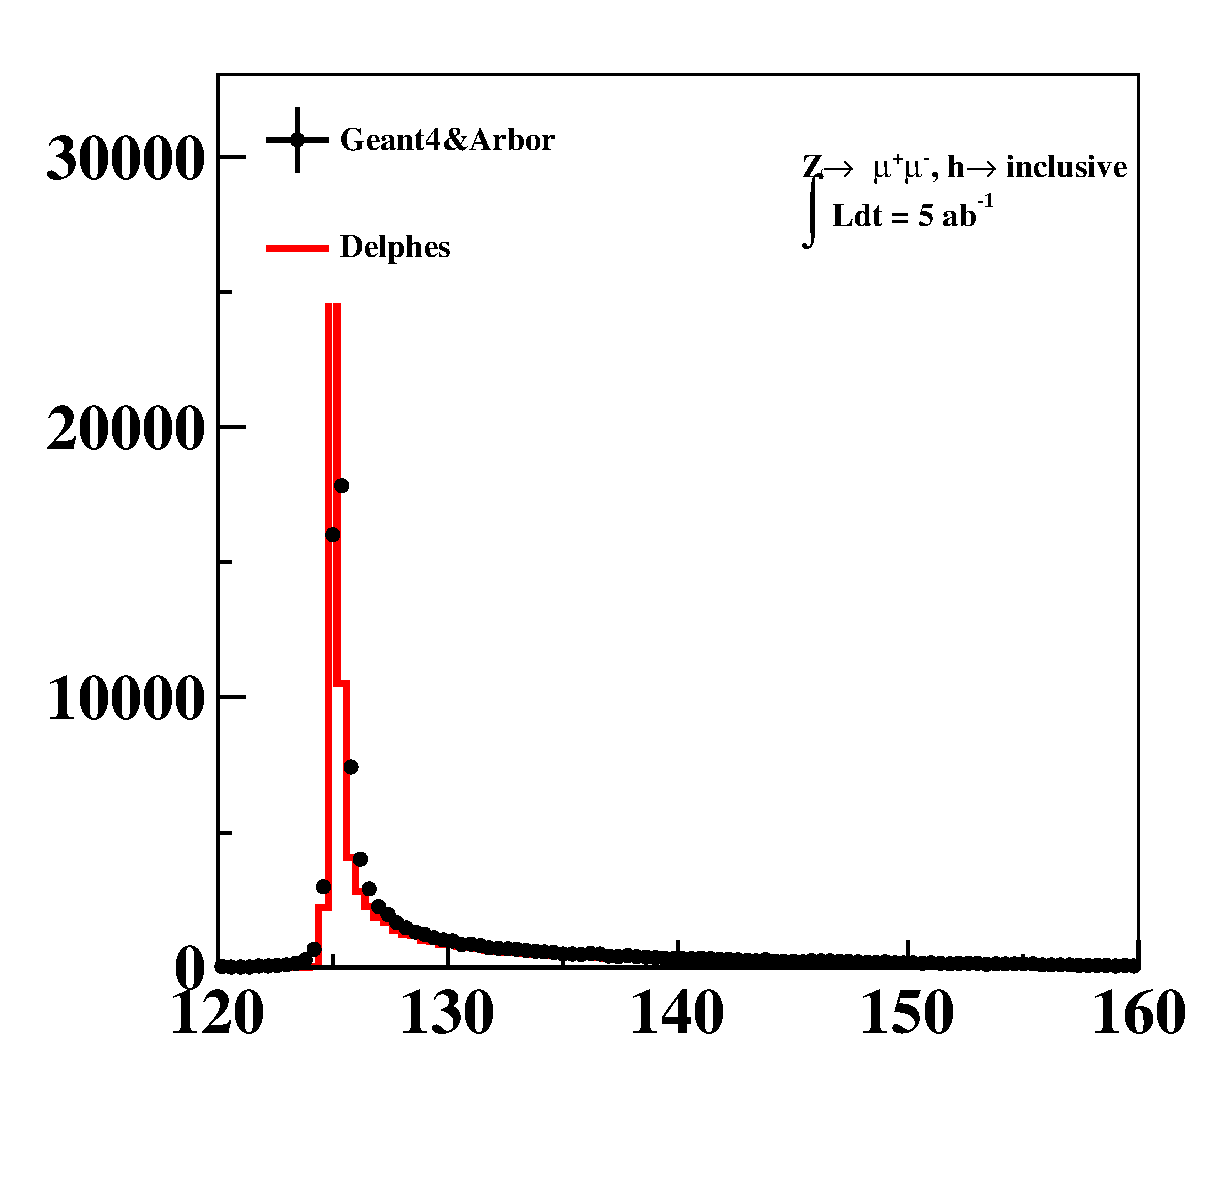
\includegraphics[width=0.9\linewidth]{e2e2h_reco}
\figcaption{\label{fig:mumureco} Recoiling mass against $\mu^+\mu^-$.}
\end{center}
\begin{center}
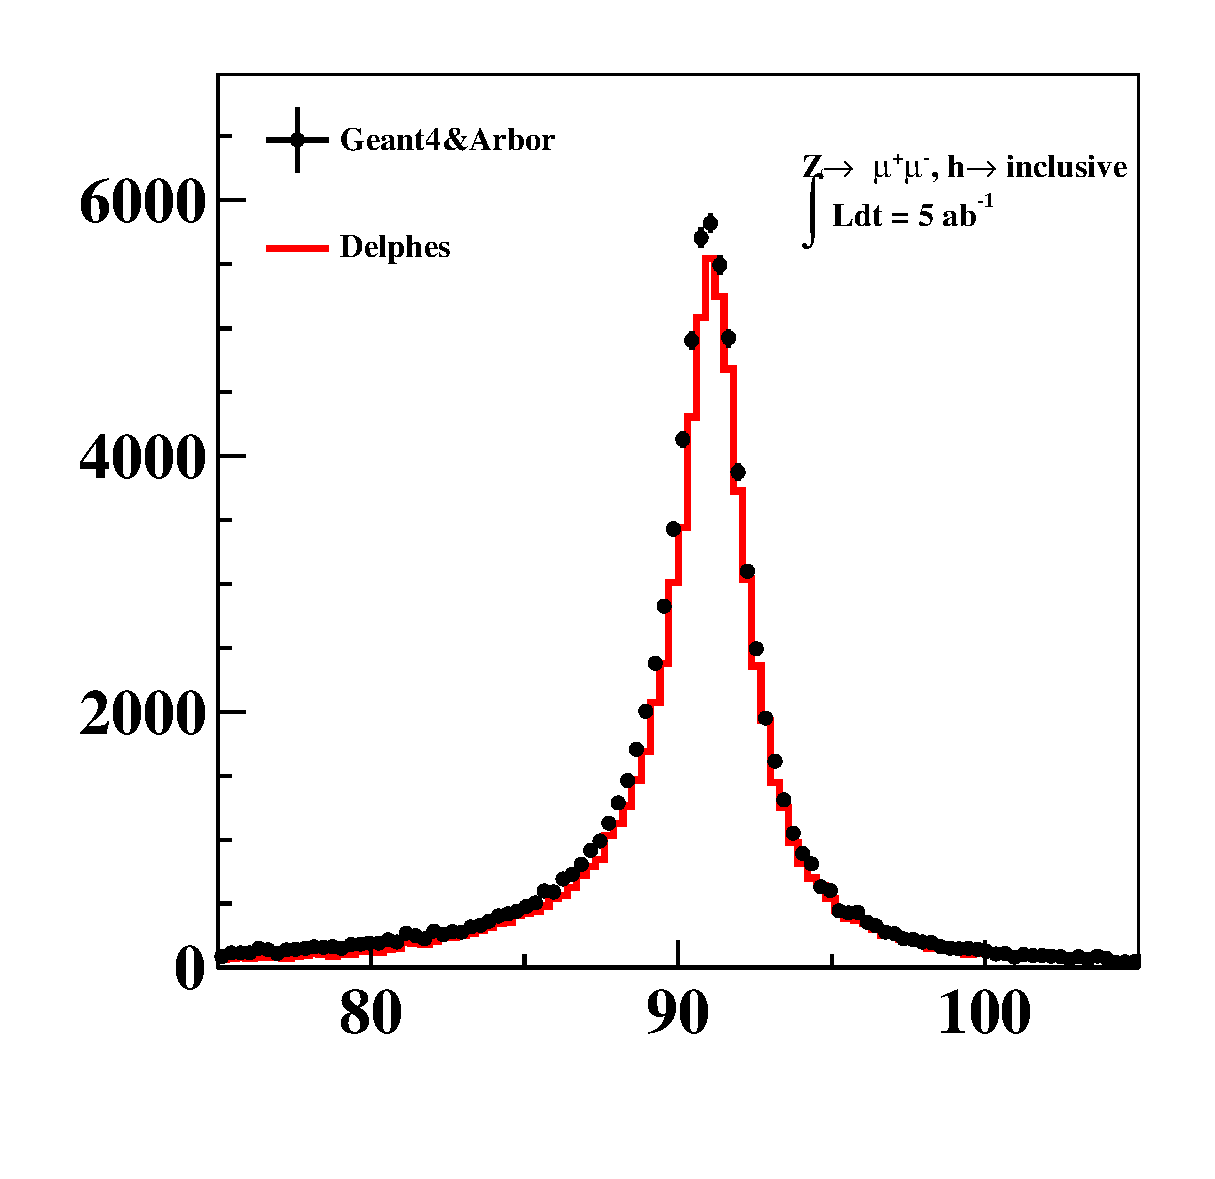
\includegraphics[width=0.9\linewidth]{e2e2h_mass}
\figcaption{\label{fig:mumuinva} Invariant mass of $\mu^+\mu^-$.}
\end{center}


\begin{center}
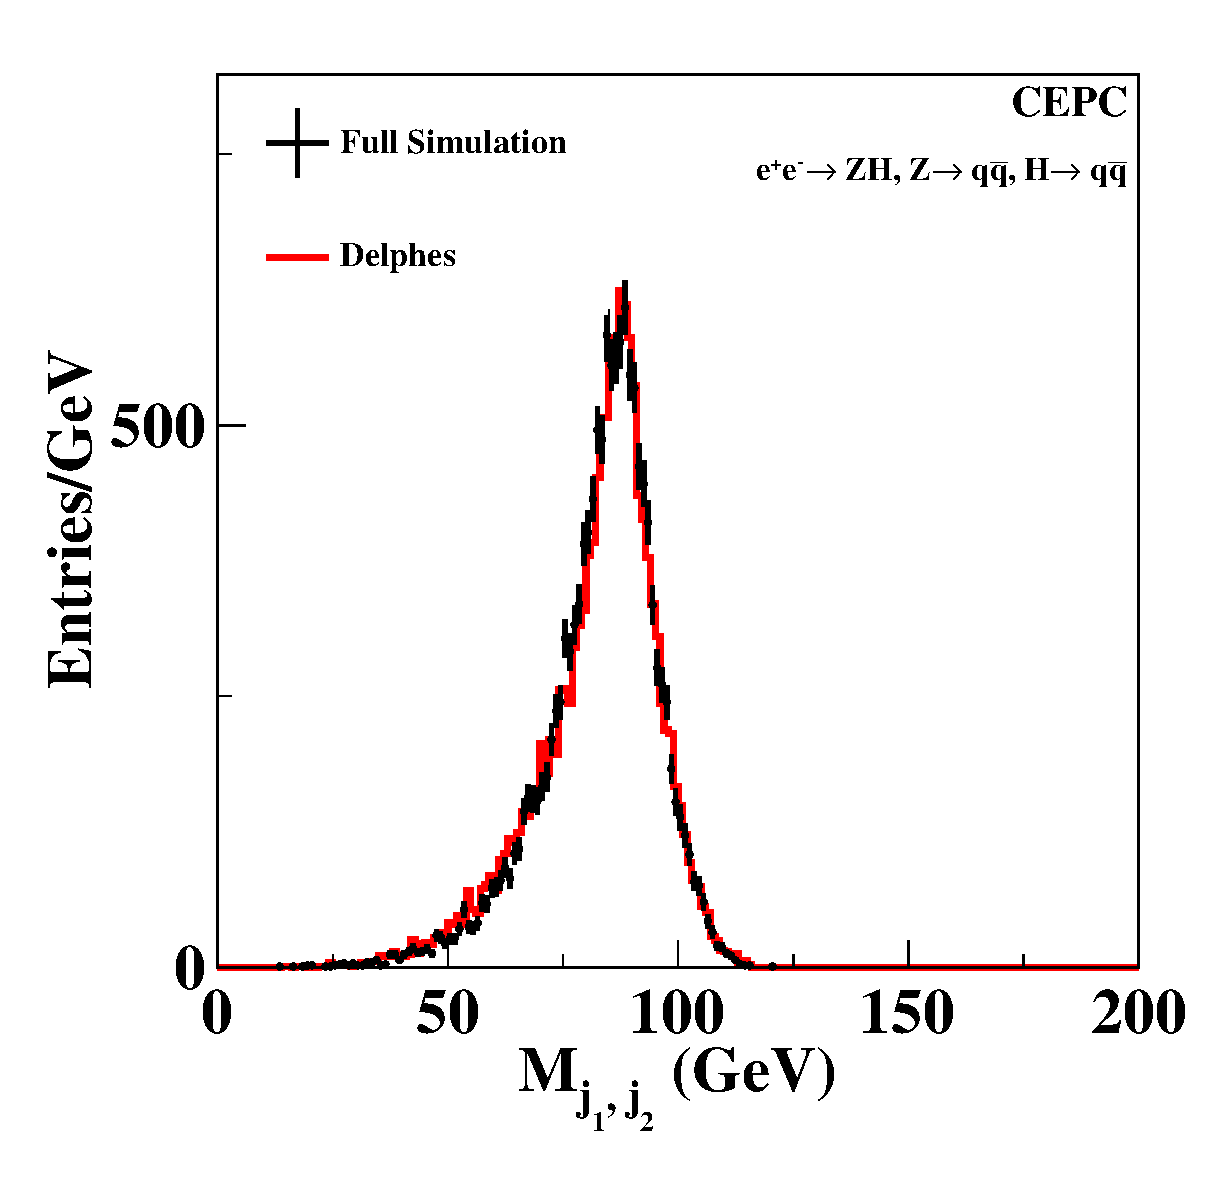
\includegraphics[width=0.9\linewidth]{full_vs_delphes_z}
\figcaption{\label{fig:zjj} Invariant mas of jet pair, peaking at $Z$ mass.}
\end{center}
\begin{center}
\includegraphics[width=0.9\linewidth]{full_vs_delphes_H}
\figcaption{\label{fig:hjj} Invariant mas of jet pair, peaking at Higgs mass}
\end{center}


\begin{center}
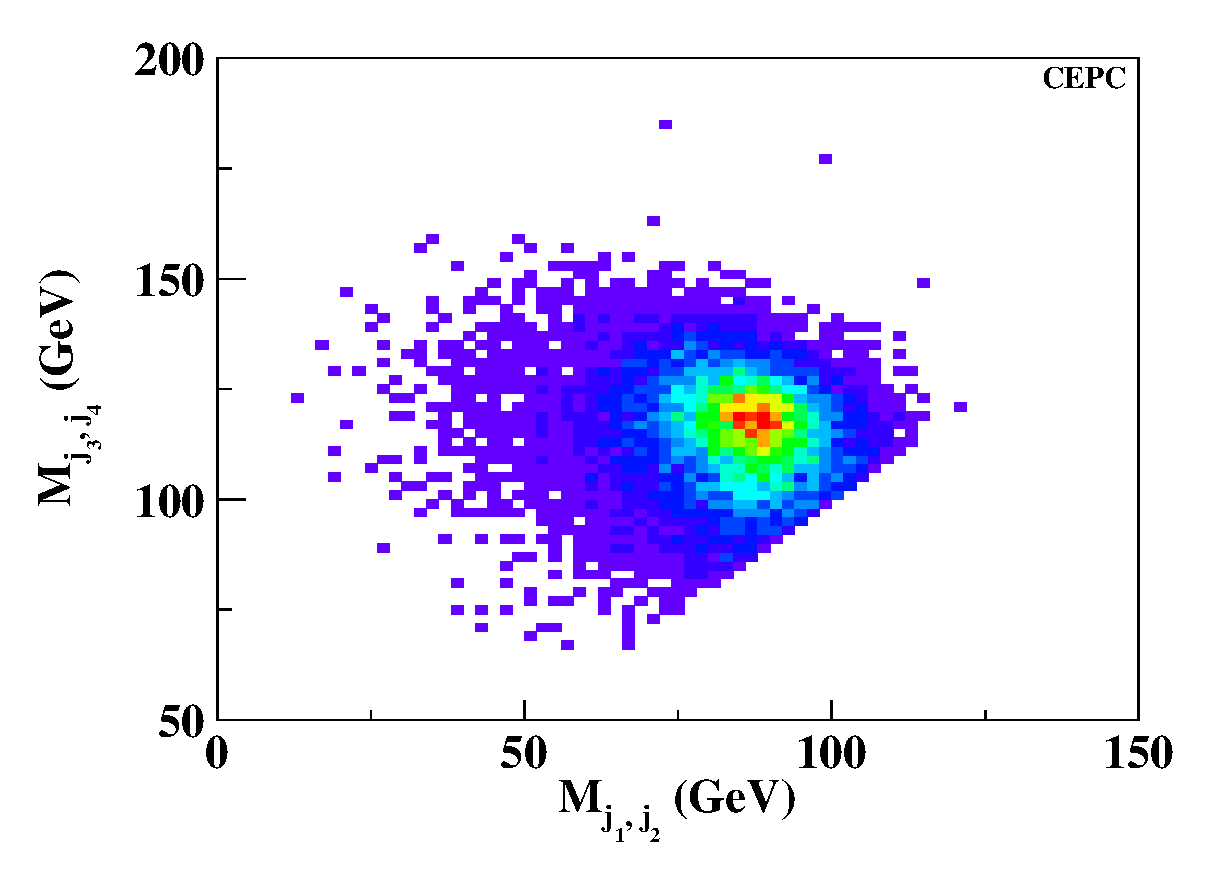
\includegraphics[width=0.9\linewidth]{Full2DCOL}
\figcaption{\label{fig:zjj} Scattering plot of $M_{j_1,j_2}$ vs. $M_{j_3,j_4}$ for full simulation}
\end{center}
\begin{center}
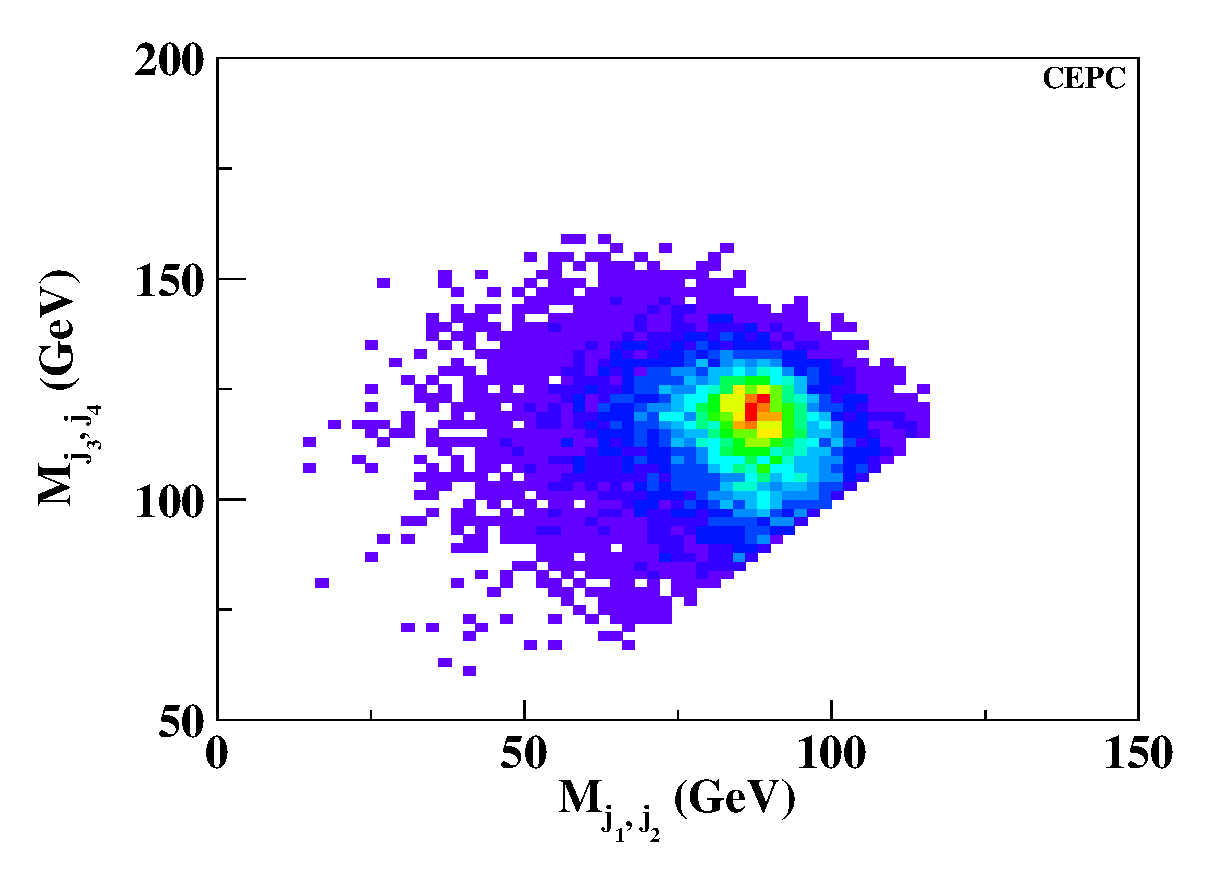
\includegraphics[width=0.9\linewidth]{Fast2DCOL}
\figcaption{\label{fig:hjj} Scattering plot of $M_{j_1,j_2}$ vs. $M_{j_3,j_4}$  for fast simulation }
\end{center}
\fi
\section{Summary and Conclusion\label{sec:summary}}

\vspace{3mm}

\begin{thebibliography}{90}
\vspace{3mm}
\bibitem{ref:1}The ATLAS Collaboration, G. Aad et al., Phys. Lett. B, 2012, {\bf 716}: 1---29.
\bibitem{ref:2}The CMS Collaboration, S. Chatrchyan et al., Phys. Lett. B, 2012, {\bf 716}: 30---61.
\bibitem{ref:ilc}T. Abe et al., The International Large Detector: Letter of Intent, arXiv:1006.3396.
\bibitem{ref:ild}T. Behnke et al., The International Linear Collider Technical Design Report --- Volume4:Detectors, arXiv:1306.6329.
\bibitem{ref:cepc_det}CEPC-SppC Preliminary Conceptual Design Report: Physics and Detector, by the CEPC Study Group (2015).
\bibitem{ref:cepc_acc}CEPC Accelerator Preliminary Conceptual Design Report, by the CEPC Study Group (2015).
\bibitem{ref:fccee} http://tlep.web.cern.ch
\bibitem{ref:clic} http://clic-study.web.cern.ch
\bibitem{ref:jiayu} 
  Q.~F.~Sun, F.~Feng, Y.~Jia and W.~L.~Sang,
  ``Mixed electroweak-QCD corrections to $e^+e^-\to HZ$ at Higgs factories,''
  arXiv:1609.03995 [hep-ph].
\bibitem{ref:yangll} 
  Y.~Gong, Z.~Li, X.~Xu, L.~L.~Yang and X.~Zhao,
  ``Mixed QCD-EW corrections for Higgs boson production at $e^+e^-$ colliders,''
  arXiv:1609.03955 [hep-ph].
\bibitem{ref:isr1}
  E.~A.~Kuraev and V.~S.~Fadin,
  Sov.\ J.\ Nucl.\ Phys.\  {\bf 41} (1985) 466
   [Yad.\ Fiz.\  {\bf 41} (1985) 733].
\bibitem{ref:isr2} 
  G.~Altarelli and G.~Martinelli,
  In *Ellis, J. ( Ed.), Peccei, R.d. ( Ed.): Physics At Lep, Vol. 1*, 47-57
\bibitem{ref:isr3} 
  O.~Nicrosini and L.~Trentadue,
  Phys.\ Lett.\ B {\bf 196}, 551 (1987).
  doi:10.1016/0370-2693(87)90819-7
\bibitem{ref:isr4} 
  F.~A.~Berends, W.~L.~van Neerven and G.~J.~H.~Burgers,
  %``Higher Order Radiative Corrections at LEP Energies,''
  Nucl.\ Phys.\ B {\bf 297}, 429 (1988)
  Erratum: [Nucl.\ Phys.\ B {\bf 304}, 921 (1988)].
\bibitem{ref:isr5} 
  F.~A.~Berends, W.~L.~van Neerven and G.~J.~H.~Burgers,
  %``Higher Order Radiative Corrections at LEP Energies,''
  Nucl.\ Phys.\ B {\bf 297}, 429 (1988)
  Erratum: [Nucl.\ Phys.\ B {\bf 304}, 921 (1988)].


\end{thebibliography}
%\end{multicols}

\clearpage

\end{document}
